\chapter{The automated hybrid surrogate-MCMC pipeline}
\label{ch:hybrid}

The procedure of \cref{ch:surrogate} works, but leaves every decision to the user and gives no
guarantee at the end. \code{slurm_mcmc_hybrid} automates it: it iterates fit, sample and validate
until measured criteria say the surrogate posterior can be trusted, recycling every expensive
evaluation it makes along the way.

\section{The loop}
\label{sec:hybrid-loop}

\begin{figure}[H]
  \centering
  \begin{tikzpicture}[
      font=\small, node distance=5mm and 9mm,
      box/.style={draw=accent, fill=accentsoft, rounded corners=2pt, align=center,
                  minimum width=44mm, minimum height=9mm, inner sep=4pt},
      cheap/.style={box, fill=white},
      test/.style={draw=accent, fill=white, diamond, aspect=2.4, align=center, inner sep=1pt},
      done/.style={box, draw=teal!60!black, fill=teal!8},
      arr/.style={-{Stealth[length=2.2mm]}, draw=accent, thick},
      lbl/.style={font=\footnotesize, text=black!70}]
    \node[box]   (r0)    {\textbf{Round 0}: short expensive MCMC\\+ regularization points};
    \node[cheap, left=of r0, minimum width=34mm] (seed) {existing evaluations\\(round 0 skipped)};
    \node[cheap, below=of r0]    (train) {training set};
    \node[cheap, below=of train] (fit)   {\textbf{fit} the surrogate};
    \node[cheap, below=of fit]   (samp)  {\textbf{sample} it: cheap chain,\\refining depth};
    \node[box,   below=of samp]  (val)   {\textbf{validate}: $N$ expensive\\evaluations on its posterior};
    \node[test,  below=of val]   (pass)  {criteria\\met?};
    \node[box,   below=of pass]  (ver)   {\textbf{verify}: re-sample to reporting\\depth, validate again};
    \node[test,  below=of ver]   (vpass) {still\\met?};
    \node[done,  below=of vpass] (out)   {return the posterior};
    \draw[arr] (r0) -- (train);
    \draw[arr] (seed) |- (train);
    \draw[arr] (train) -- (fit);
    \draw[arr] (fit) -- (samp);
    \draw[arr] (samp) -- (val);
    \draw[arr] (val) -- (pass);
    \draw[arr] (pass) -- node[lbl, right] {yes} (ver);
    \draw[arr] (ver) -- (vpass);
    \draw[arr] (vpass) -- node[lbl, right] {yes} (out);
    \coordinate (back) at ($(train.east)+(22mm,0)$);
    \draw[arr] (pass.east) -- node[lbl, above, pos=0.35] {no} (pass.east -| back) -- (back) -- (train.east);
    \draw[arr] (vpass.east) -- node[lbl, above, pos=0.35] {no} (vpass.east -| back) -- (pass.east -| back);
    \node[lbl, align=left, anchor=west] at ($(back)!0.5!(pass.east -| back) + (1.5mm,0)$)
      {validation points\\join the\\training set};
  \end{tikzpicture}
  \caption{The loop. Shaded boxes spend expensive evaluations, white boxes only cheap ones. Every
           expensive evaluation, including those of a verification, ends up in the training set.}
  \label{fig:hybrid-loop}
\end{figure}

\begin{enumerate}[leftmargin=*, label=\textbf{\arabic*.}]
  \item \textbf{Round 0.} A \emph{short} expensive MCMC, plus optional
        \code{num_regularization_points}, generates the initial training set. Its walkers --- the
        parallel MCMC chains of \cref{ch:mcmc} --- are evaluated in parallel on the cluster, so
        their number is this stage's parallelism. The regularization points are the only
        evaluations in the whole run placed without reference to a posterior, and so the only ones
        that can find mass the surrogate does not already know about.
  \item \textbf{Fit} a fast surrogate: a Gaussian process by default (\cref{sec:hybrid-surrogates}).
  \item \textbf{Sample} the surrogate with a cheap, vectorized MCMC that needs no cluster, confined
        to \code{param_bounds} or, by default, to an envelope grown from the training data
        (\cref{sec:unbounded}). A fresh sampler is built every round, because each round samples a
        different surrogate, with its own deliberately small set of walkers. This chain is kept
        cheap, because its posterior is discarded at the next fit.
  \item \textbf{Validate.} Evaluate the expensive function, in parallel, on
        \code{num_validation_points} drawn from the surrogate posterior, and score the criteria of
        \cref{sec:hybrid-measured}.
  \item \textbf{Refine.} If the criteria are not met, the validation evaluations --- which sit
        exactly where the surrogate needs improving, and are already paid for --- join the training
        set, and the loop returns to step 2. Optionally, each round also runs a few expensive MCMC
        steps started from the current surrogate posterior (\code{num_expensive_iters_per_round}).
  \item \textbf{Verify.} A pass reached on a cheap chain is only provisional. The same surrogate is
        re-sampled to reporting depth (\cref{sec:two-depths}) and one more validation batch is
        spent on \emph{that} posterior. If it still passes, it is the posterior returned; if not,
        refinement resumes. No evaluation is wasted either way: the refinement batch joins the
        training set as soon as verification starts, and a rejected verification's batch joins it
        too.
\end{enumerate}

Verification buys two things. The returned posterior is sampled properly, rather than being
whatever a deliberately cheap chain happened to produce. And the decision to stop rests on two
independent measurements rather than one --- which matters, because a single measurement from 100
validation batch is noisy: two batches scored against the \emph{same} surrogate can land on opposite
sides of the threshold.

\begin{keypoint}[Starting from existing evaluations]
If expensive evaluations already exist --- from an ordinary \code{slurm_mcmc} run, a parameter scan,
an earlier study --- pass them as \code{initial_train_points} and \code{initial_train_values}. Round 0
is skipped and the first surrogate is fitted on them directly; \code{init_points} is then not needed,
and the evaluations do not count towards \code{num_expensive_evals}, which records only what the run
itself spent. The regularization points are part of round 0, so they are skipped too, with a warning.
A typical source is an earlier plain \code{slurm_mcmc} on the expensive function that was taking too
long to converge: stop it, and hand its whole history to the hybrid pipeline, so that none of the
evaluations it has already paid for is wasted.
\begin{lstlisting}
pool = status['slurm_pool']                 # from a previous slurm_mcmc
result = slurm_mcmc_hybrid(..., initial_train_points=pool.points_history,
                           initial_train_values=pool.values_history[:, 0])
\end{lstlisting}
\end{keypoint}

\section{What is measured}
\label{sec:hybrid-measured}

On the validation points $\theta_i$, write the log-ratio of the expensive to the surrogate
log-probability, and the self-normalised importance weights of \cref{sec:importance}:
\begin{equation}
  d_i = \log\pexp(\theta_i) - \log\psur(\theta_i),
  \qquad w_i = e^{d_i},
  \qquad \tilde w_i = \frac{w_i}{\sum_j w_j}.
\end{equation}
The weights are the \emph{ratio}, not the expensive density, because the points were drawn from the
surrogate posterior and so already arrive with density $\propto \psur$: the sampling density has to
be divided out before the target density is multiplied in.

\begin{keypoint}[Nats]
Every logarithm here is natural, and the unit of a log-probability is the \emph{nat} --- which is
what ``[nats]'' means on the figures below. A difference of $\Delta$ nats in log-probability is a
factor $e^{\Delta}$ in probability: 1~nat is a factor of 2.7, 0.1~nats about 10\%, and 0.01~nats
about 1\%.
\end{keypoint}

\subsection{Surrogate accuracy}

\begin{equation}
  \bar d = \sum_i \tilde w_i\, d_i,
  \qquad
  \varepsilon = \sqrt{\sum_i \tilde w_i\, (d_i - \bar d)^2}\quad[\text{nats}].
  \label{eq:epsilon}
\end{equation}
$\varepsilon = 0.05$ means probability ratios are accurate to about 5\%. The mean $\bar d$ is
subtracted because a log-probability is only defined up to a constant, so only the \emph{spread} of
$d$ is a real error. The weighting makes $\varepsilon$ an average under the \emph{expensive}
posterior: an error where the true probability is high counts far more than the same error in the
tails.

\subsection{Weight efficiency}

$\varepsilon$ alone is not safe, for two reasons. First, if the weights collapse onto a few points,
$\varepsilon$ is computed from those points alone and can be arbitrarily small --- exactly zero for a
single dominating point --- while the surrogate is in fact terrible. Second, and more commonly, the
weighting that makes $\varepsilon$ an average under the expensive posterior also makes it blind to
surrogate mass where the expensive posterior has none: a validation point with $d_i \ll 0$ gets
$w_i \approx 0$ and drops out of \cref{eq:epsilon}. A surrogate posterior with a spurious lobe, or
with tails far too wide, can therefore pass the accuracy test while a large fraction of the samples
it reports are wrong. Both failures show in how evenly the weights are spread, measured by the
\emph{weight efficiency} --- the importance-sampling (Kish) efficiency of the $N$ validation points:
\begin{equation}
  \effw = \frac{\left(\sum_i w_i\right)^2}{N\sum_i w_i^2} \in \left[\tfrac{1}{N},\, 1\right].
  \label{eq:weight-efficiency}
\end{equation}
$N\effw$ is the number of validation points that effectively carry the weight. If a fraction $s$ of
the surrogate posterior lies where the expensive one is negligible, and the rest is accurate,
$\effw \approx 1 - s$, so a floor on $\effw$ is a bound on the junk fraction of the reported
posterior. When $d$ is roughly Gaussian with spread $\varepsilon$, $\effw \approx e^{-\varepsilon^2}$:
$0.99$ at the default $\varepsilon^\ast = 0.1$, so a genuinely converged surrogate clears the default
floor \code{min_weight_efficiency}$\,= 0.9$ easily, while a surrogate with more than about 10\% of its
mass in the wrong place, or with a few dominating points, never converges. The floor is equivalent
to $\varepsilon \lesssim 0.32$ for Gaussian errors, so with a looser \code{log_error_threshold} than
that it becomes the binding criterion. Its resolution is set by $N$: the scatter of $\effw$ near
$0.9$ is about $\sqrt{0.09/N}$, $0.02$ at $N = 200$, which is one reason for the floor of 200 in the
default \code{num_validation_points}. $\effw$ is printed per round as the \code{w_eff} column of the
diagnostics (\cref{sec:hybrid-diagnostics}).

\subsection{Posterior stability}

Surrogate accuracy and posterior convergence are different questions: a perfect surrogate still
leaves a drifting posterior if its chain is too short. Between rounds, the change in each
parameter's posterior mean $m_j$ and standard deviation $s_j$ is measured in units of that
parameter's posterior width, and the largest is kept:
\begin{equation}
  \delta = \max_j
  \frac{\max\!\left(\,\big|m_j^{\mathrm{new}} - m_j^{\mathrm{old}}\big|,\ \big|s_j^{\mathrm{new}} - s_j^{\mathrm{old}}\big|\,\right)}
       {\tfrac12\left(s_j^{\mathrm{new}} + s_j^{\mathrm{old}}\right)} .
  \label{eq:delta}
\end{equation}
$\delta = 0.1$ means nothing moved by more than a tenth of a posterior width --- a statement about
the answer rather than about the chain. Two estimates of the \emph{same} posterior still differ by
chance, by roughly $\sqrt{1/\ESS_{\mathrm{new}} + 1/\ESS_{\mathrm{old}}}$ widths, where ESS is the
chain's and ``old'' is the previous round's reported posterior. The tolerance actually applied
therefore never drops below three times that noise floor:
\begin{equation}
  \delta \;\le\; \max\!\left(\texttt{posterior\_shift\_tolerance},\;
  3\sqrt{\frac{1}{\ESS_{\mathrm{new}}} + \frac{1}{\ESS_{\mathrm{old}}}}\right).
  \label{eq:stability}
\end{equation}
Without the floor a tolerance of 0.1 would be unreachable at realistic chain depths: at the ESS of
95--380 in the worked example, the floor alone is 0.23--0.42. The test needs two rounds, so a run
cannot converge in round 1 while it is enabled. It is off by default
(\code{posterior_shift_tolerance=None}), which keeps the test to accuracy and weight efficiency;
setting it, e.g. to 0.1, also requires the posterior to have stopped moving, which catches a surrogate
that is accurate on its current posterior but still improving between rounds.

\subsection{The convergence test}

All the conditions enabled must hold simultaneously; the third only when
\code{posterior_shift_tolerance} is set:
\begin{gather}
  \varepsilon \le \texttt{log\_error\_threshold},
  \qquad
  \effw \ge \texttt{min\_weight\_efficiency},
  \notag\\
  \delta \le \max\!\left(\texttt{posterior\_shift\_tolerance},\ \text{noise floor}\right).
\end{gather}

\begin{cautionbox}[What the test cannot see]
Every statistic is evaluated on points drawn from the \emph{surrogate} posterior. The test therefore
detects a surrogate posterior that is too \textbf{broad}, and cannot detect one that is too
\textbf{narrow}: mass the surrogate never finds is never sampled, never scored, and never enters any
statistic. The worked example below misses a tail in exactly this way. If the target may be
hierarchical or multimodal, spend some budget on \code{num_regularization_points}, disperse
\code{init_points}, and consider an independent short expensive chain as a check.
\end{cautionbox}

\section{Two sampling depths}
\label{sec:two-depths}

The two chain criteria of \cref{sec:mcmc-convergence} are applied at two depths. Once the
autocorrelation time $\tau$ is known, the floors of a depth fix the chain length it needs: with $\Nc$
walkers and a burn-in fraction $b$, $\ESS = \Nc(1-b)\Lc/\tau$, so
\begin{equation}
  \Lc \;\ge\; \max\!\left(\frac{\ESS_{\min}\,\tau}{\Nc(1-b)},\ (\Lc/\tau)_{\min}\,\tau\right).
  \label{eq:chain-length}
\end{equation}
$\tau$ depends strongly on the target and is not known in advance, but it is measured on every chain.
By default (\code{num_surrogate_iters='auto'}) each chain is therefore sized from a $\tau$ already
measured, and starts 20\% past the length \cref{eq:chain-length} gives for it. A refining chain takes
the $\tau$ of the chain before it. A verifying chain takes the largest $\tau$ of the run: the
refining chain before it is too short to measure $\tau$ well, and $\tau$ measured on a short chain is
biased low. Only the first chain of a run starts from a guess, $\tau = 10\,d$, a typical value for
the stretch move on a well-shaped posterior. The chain is then extended, on the same sampler, to the
length \cref{eq:chain-length} gives for its re-measured $\tau$, until the floors of its depth hold.

Some posteriors never let it get there: when the walkers visit a long arm rarely and stay a long
time, $\tau$ keeps growing with the chain, and $\Lc/\tau$ does not rise however long the chain is. A
chain whose $\Lc/\tau$ has not risen over two extensions in a row is therefore stopped, with a
warning, and \code{max_surrogate_iters} ($10^6$ by default) caps every chain as a last resort. A
verification whose chain stops short of its floors is never accepted, since its effective sample
size is overstated and its stability test too lenient; it is recorded as blocked by
\code{chain-depth}. When a target's slow direction puts the verification floors out of reach,
lowering \code{verify_iters_per_tau} or \code{verify_surrogate_ess} is a deliberate choice, made
visible in the settings. An integer \code{num_surrogate_iters} fixes only the starting length.

\begin{center}
\small
\begin{tabularx}{\linewidth}{@{}l L L@{}}
  \toprule
  & \textbf{refining} --- posterior discarded at the next fit & \textbf{verifying} --- posterior reported \\
  \midrule
  effective samples, $N/\tau$ & \code{refine_surrogate_ess}: \code{'auto'} $\to 10\,d$ & \code{verify_surrogate_ess}: \code{'auto'} $\to 100\,d$ \\
  chain length, $\Lc/\tau$    & \code{refine_iters_per_tau}: \code{'auto'} $\to 10$ & \code{verify_iters_per_tau}: \code{'auto'} $\to 50$ \\
  \bottomrule
\end{tabularx}
\end{center}

The ESS defaults are the two ends of the advised band of $10$--$100\times d$. The length floors
differ in purpose. While refining, $\Lc \ge 10\tau$ is only the shortest chain whose own $\tau$ can be
estimated at all (\texttt{emcee}'s window takes $5\tau$); the posterior is discarded at the next fit, so
nothing more is asked. While verifying, $\Lc \ge 50\tau$ is \texttt{emcee}'s rule for a reliable $\tau$,
since that posterior is the one reported. \code{None} switches either floor off. Samples and $\tau$
are always taken after discarding \code{surrogate_burnin_fraction} of the chain.

\code{max_verification_attempts}, by default \code{None}, lets a failed verification send the run
back to refining as often as the target needs, since \code{num_rounds_max} bounds it anyway. A finite
cap means \emph{give up after this many rejections} and ends the run: a run that can no longer
verify can never converge. \code{0} switches verification off.

\section{Surrogate models}
\label{sec:hybrid-surrogates}

\code{surrogate} accepts one of the following, or any object with \code{fit(X, y)} and
\code{predict(X)} --- and \code{predict_std(X)} too, if the uncertainty penalty should be active:

\begin{itemize}
  \item \textbf{\code{'gp'}} (default), a \code{GaussianProcessSurrogate} --- the recommended choice:
        accurate, smooth, and it reports its own uncertainty.
  \item \textbf{\code{'polynomial'}}, a \code{PolynomialSurrogate} --- a cheap fallback for
        posteriors that really are low-order. It extrapolates badly otherwise, and has no
        uncertainty, so the uncertainty penalty is inactive with it.
  \item \textbf{\code{DistributedGPSurrogate(...)}} --- an ensemble of Gaussian processes, for when
        the training set has grown too large for a single one to be refitted every round.
\end{itemize}

The first two wrap standard scikit-learn models:
\code{GaussianProcessRegressor} for the Gaussian process, and a ridge regression on polynomial
features for the polynomial. The Gaussian process first fits a polynomial mean function, so that the
process only has to model what the polynomial misses. The third,
\code{DistributedGPSurrogate}, is not a standard model, and is described in \cref{sec:rbcm}.

\subsection{The uncertainty penalty}

During the surrogate MCMC the surrogate is evaluated pessimistically, as
\begin{equation}
  \log\psur(\theta) = \mu(\theta) - \kappa\, \sigma(\theta),
\end{equation}
where $\mu$ and $\sigma$ are its prediction and uncertainty and $\kappa$ is
\code{surrogate_uncertainty_penalty}. A Gaussian process's uncertainty grows away from its training
data, so walkers are turned back from regions where the surrogate would be extrapolating.

\subsection{DistributedGPSurrogate}
\label{sec:rbcm}

\textbf{Why it exists.} The surrogate is refitted every round on the whole training set, and the
cost of fitting a Gaussian process grows steeply --- roughly with the cube of the number of points.
Early in a run that is negligible, but every round adds evaluations, so on a long run the fit comes
to dominate and eventually stops being affordable at all. \code{DistributedGPSurrogate} is the way
past that point.

\textbf{What it does.} It is a robust Bayesian Committee Machine (Deisenroth \& Ng 2015, with Cao \&
Fleet's 2014 weights). It splits the training set among independent Gaussian-process
\emph{experts} and recombines their predictions in closed form. It attacks cost by parallelism
rather than approximation: the expert fits are independent, so on a cluster the wall clock is that of
a single expert.

At any point, every expert predicts a value and an uncertainty, and the ensemble takes a weighted
average of the values. An expert's weight is how much it has learned at that point: how far its
uncertainty there has fallen below the uncertainty it had before seeing any data. An expert sitting
on its own training points is confident and dominates; an expert far from them is back where it
started and gets no weight at all. The weights add up to one, so a single expert reproduces itself
exactly --- a one-expert ensemble \emph{is} the dense Gaussian process --- and where no expert has
learned anything, the ensemble falls back to the experts' starting uncertainty, which is large. That
large uncertainty is what keeps the uncertainty penalty working away from the data. Each expert is
judged against the uncertainty \emph{it} started with: experts routinely settle on scales far from
the nominal one, and judging them against it would make every expert look uninformed away from its
data.

\begin{argtable}
  \code{max_points_per_expert} & \code{None} & set this for large training sets: it grows the \emph{number} of experts with the data instead of the size of each, which keeps fitting affordable \\
  \code{num_experts} & \code{8} & the number of experts, when \code{max_points_per_expert} is not set \\
  \code{min_points_per_expert} & \code{200} & below this many points per expert, fewer experts are used, down to one; an expert fitted on a few dozen points cannot identify its own kernel \\
  \code{partition} & \code{'kmeans'} & how points are split: \code{'kmeans'} (spatial clusters) or \code{'random'} \\
  \code{n_restarts_optimizer} & \code{2} & restarts of each expert's hyperparameter fit; more give better fits for little cost \\
  \code{parallel} & \code{'none'} & \code{'joblib'}: one process per core; \code{'slurm'}: one job array across nodes, worth it only when a single expert fit is long compared with the queue wait \\
  \code{n_jobs}, \code{cluster}, \code{submitit_kwargs} & \code{-1}, \code{'slurm'}, \code{None} & settings of the \code{'joblib'} and \code{'slurm'} modes \\
  \code{work_dir} & \code{None} & scratch location for \code{'slurm'}, \code{work_dir/surrogates/dgp_experts}, removed once the experts are back; inherited from the pipeline's, and must be on a shared filesystem \\
  \code{job_name} & \code{None} & for \code{'slurm'}, the expert job arrays are named \code{job_name_dgp_fit<n>}; inherited from the pipeline's \\
  \code{max_fit_retries} & \code{2} & failed expert jobs are retried individually, then fitted locally \\
  \code{trend_degree} & \code{2} & the polynomial mean function, as for the dense Gaussian process \\
\end{argtable}

Two behaviours are worth knowing. The prediction cannot be computed without the uncertainties,
because the weights come from them, so turning the uncertainty penalty off saves the ensemble
nothing. And cost moves rather than disappears: every MCMC step queries all the experts, so fitting
becomes nearly free while sampling becomes the dominant cost, and end to end the ensemble can be
slower than the dense Gaussian process even though it fits far faster. It pays once the dense fit
itself is the bottleneck.

\section{Training data}

The training set only grows: every expensive evaluation is kept. What enters each fit can be
limited. \code{train_log_prob_trim_range} drops points more than that many nats below the best
one --- their probability is $e^{-100}$ at the default, so no MCMC will ever visit them, and they only
make the fit more expensive. The trim is skipped in any round where it would leave fewer than
\code{min_train_points_after_trim} points, $10\,d$ by default: early on, a single lucky evaluation far
above the rest would otherwise trim the training set to a handful of points.
Below about 20 nats accuracy collapses, because the surrogate then has no evidence that the
probability is low away from the peak. \code{max_train_points} caps the fit with a uniform random
subsample, which preserves spatial coverage; keeping the highest-probability points instead would
discard exactly the far-field points that stop the surrogate extrapolating. \code{train_log_prob_floor}
drops points below an absolute value, such as penalty or failure values.

\section{Running without bounds}
\label{sec:unbounded}

\code{param_bounds} defaults to \code{None}, and then no box is imposed. A box cannot simply be
dropped, though, because a surrogate says nothing reliable away from its training data, and both ways
it can be wrong there are fatal to an MCMC: with a fitted quadratic trend the surrogate tends to that
quadratic, which runs off to $+\infty$ along any direction of positive curvature; without a trend it
tends to a constant, which is improper over infinite volume. Either way the chain walks away and
never returns.

So the training set's own geometry decides where the surrogate may be believed. Let $r(\theta)$ be
the Mahalanobis radius of $\theta$ under the training points' mean and covariance, and $R$ the largest
such radius among them. A quartic penalty switches on beyond $2R$, and the log-probability is
$-\infty$ beyond $10R$, which makes the posterior proper outright. Nothing acts inside $2R$, so the
posterior over the data is untouched; and because both radii are multiples of $R$, they grow as
evaluations accumulate outwards, so a genuinely long tail is followed round after round.

With the default Gaussian process the envelope never actually fires: its uncertainty grows away from
the data, so the uncertainty penalty turns the walkers back long before the envelope --- on the
worked example, the largest radius the walkers reached was 3.51 with the envelope switched on and off
alike. It is load-bearing only for surrogates without an uncertainty, such as the polynomial.

\needspace{22\baselineskip}
\section{Usage}
\label{sec:hybrid-usage}

\begin{lstlisting}
import numpy as np
from slurmcmc.hybrid import slurm_mcmc_hybrid

def log_prob(theta):                            # the expensive log-probability
    ...

num_params = 3
init_points = np.random.uniform(-2, 2, (10 * num_params, num_params))   # round-0 walkers

result = slurm_mcmc_hybrid(log_prob_fun=log_prob, init_points=init_points,
                           num_expensive_iters=10, num_regularization_points=50,
                           log_error_threshold=0.01, num_rounds_max=30,
                           cluster='slurm', work_dir='hybrid',
                           save_restart=True, random_seed=0)

print(result['converged'], result['num_rounds'], result['num_expensive_evals'])
samples = result['samples']                     # the posterior, as flat draws
\end{lstlisting}

Most arguments can stay at their defaults. The ones that decide a run are its round-0 budget ---
the number of walkers in \code{init_points}, \code{num_expensive_iters} and
\code{num_regularization_points} --- the accuracy it must reach, \code{log_error_threshold}, and
how many rounds it may take, \code{num_rounds_max}. To start from evaluations that already exist,
pass \code{initial_train_points} and \code{initial_train_values} instead of \code{init_points}
(\cref{sec:hybrid-loop}); to use another surrogate, pass \code{surrogate}
(\cref{sec:hybrid-surrogates}). With \code{remote=True} the call returns a submitit job, and
\code{result = job.result()} gives the same dictionary (\cref{sec:remote}).

\code{example_mcmc_hybrid.py} spells out every argument on its own line and is the best starting
point for a real problem; \cref{sec:hybrid-args} describes them all, and the returned dictionary is
described at the end of this chapter.

\section{Worked example: a 3D Rosenbrock}
\label{sec:hybrid-example}

This is what \code{example_mcmc_hybrid.py} does, with the settings below, so every number in this
section is reproducible by running it. The target is minus the 3D Rosenbrock function of
\cref{eq:rosenbrock}: a narrow, curved, banana-shaped posterior. Because it is analytic, a plain
expensive MCMC on it is affordable, and that gives a reference to judge the hybrid run against ---
so the reference comes first.

\subsection{The expensive reference}

The reference is a plain \code{slurm_mcmc} on the same target, with no surrogate anywhere: 100\,000
iterations with 30 walkers, \textbf{3\,000\,000 evaluations}. It is cached separately from the
pipeline's results, so changing a hybrid setting does not pay for it again. A reference is only a
yardstick once it has converged itself, so the example draws its posterior at five points along the
chain, after discarding the first 20\% as burn-in.

\begin{figure}[H]
  \centering
  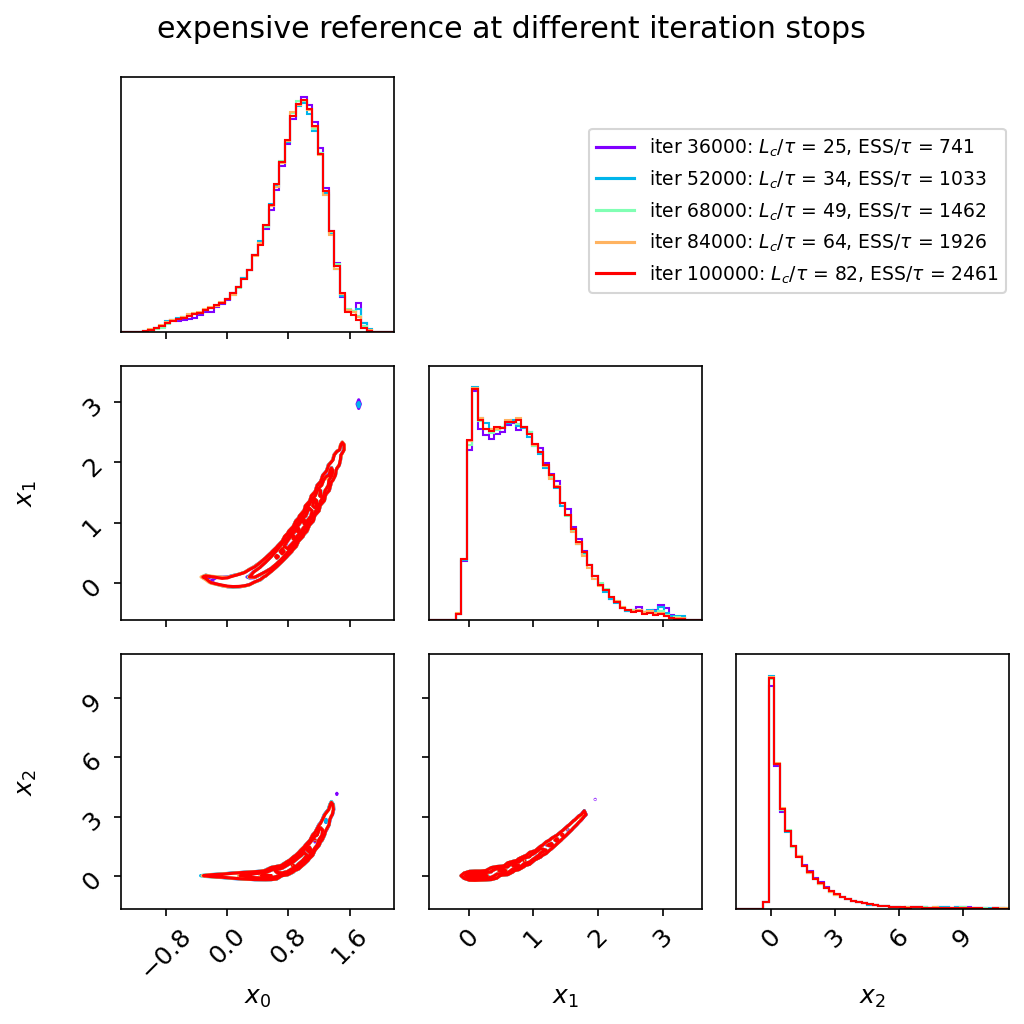
\includegraphics[width=0.5\linewidth]{example_mcmc_hybrid_reference_convergence.png}
  \caption{The reference posterior at five stopping points along the chain, with $\Lc/\tau$ and
           the effective sample size for each in the legend. The figures label the effective sample
           size ESS/$\tau$, for the number of samples divided by $\tau$; $\tau$ is the largest over
           the parameters.}
  \label{fig:hybrid-reference}
\end{figure}

The distributions agree at every stop, and $\Lc/\tau$ grows from 25 to 82. That growth is only
meaningful because $\tau$ has stopped growing (\cref{sec:mcmc-convergence}): it settles at about
850--1\,000 from the third stop on. The slowest part of the posterior is its arm at negative $x_0$,
which holds 7.4\% of the mass; walkers enter it rarely, and the longest single visit lasts 3\,511
iterations, well inside the chain.

\subsection{The hybrid run}

A \code{DistributedGPSurrogate} with the default quadratic mean function. The settings that differ
from the library defaults:

\begin{center}
\small
\begin{tabularx}{\linewidth}{@{}>{\raggedright\arraybackslash}p{0.40\linewidth}>{\raggedright\arraybackslash}p{0.17\linewidth}L@{}}
  \toprule
  \textbf{setting} & \textbf{value} & \textbf{why} \\
  \midrule
  \code{surrogate} & \code{DistributedGP} & experts of at most 500 points, fitted in parallel (\code{parallel='joblib'}) \\
  expensive walkers, \code{len(init_points)} & $10\,d = 30$ & the cluster parallelism of the expensive stage \\
  \code{num_expensive_iters}, \code{num_regularization_points} & 10, 50 & a deliberately small round-0 budget, so refinement has work to do \\
  \code{num_rounds_max} & 30 & a tighter cap than the default 100, to bound the example's cost \\
  \code{save_posterior_samples} & 2\,000 & keeps each round's posterior \\
  \bottomrule
\end{tabularx}
\end{center}

Everything else is at its default, including $\varepsilon \le 0.1$ nats, $\effw \ge 0.9$, no
posterior-shift test (\code{posterior_shift_tolerance=None}), chains sized from $\tau$, and 200
validation points per round (\code{'auto'}, $\max(200, 10\,d)$).

\begin{keypoint}[Result]
Converged in \textbf{4 rounds on 1\,580 expensive evaluations}, about 15 minutes --- 0.05\% of the
reference's evaluations. Two verifications were run; the first was rejected.
\end{keypoint}

\subsection{Convergence, round by round}

A verified round has \textbf{two rows}: $n$ for the refinement chain, whose metrics passed and so
triggered the verification, and $n$v for the verification chain that then judged it. $n_{\mathrm{exp}}$
counts the expensive evaluations accumulated before the round, and $n_{\mathrm{train}}$ those that
entered the fit; the two rows share one fit, so both are given on the first row only.

\begin{figure}[H]
  \centering
  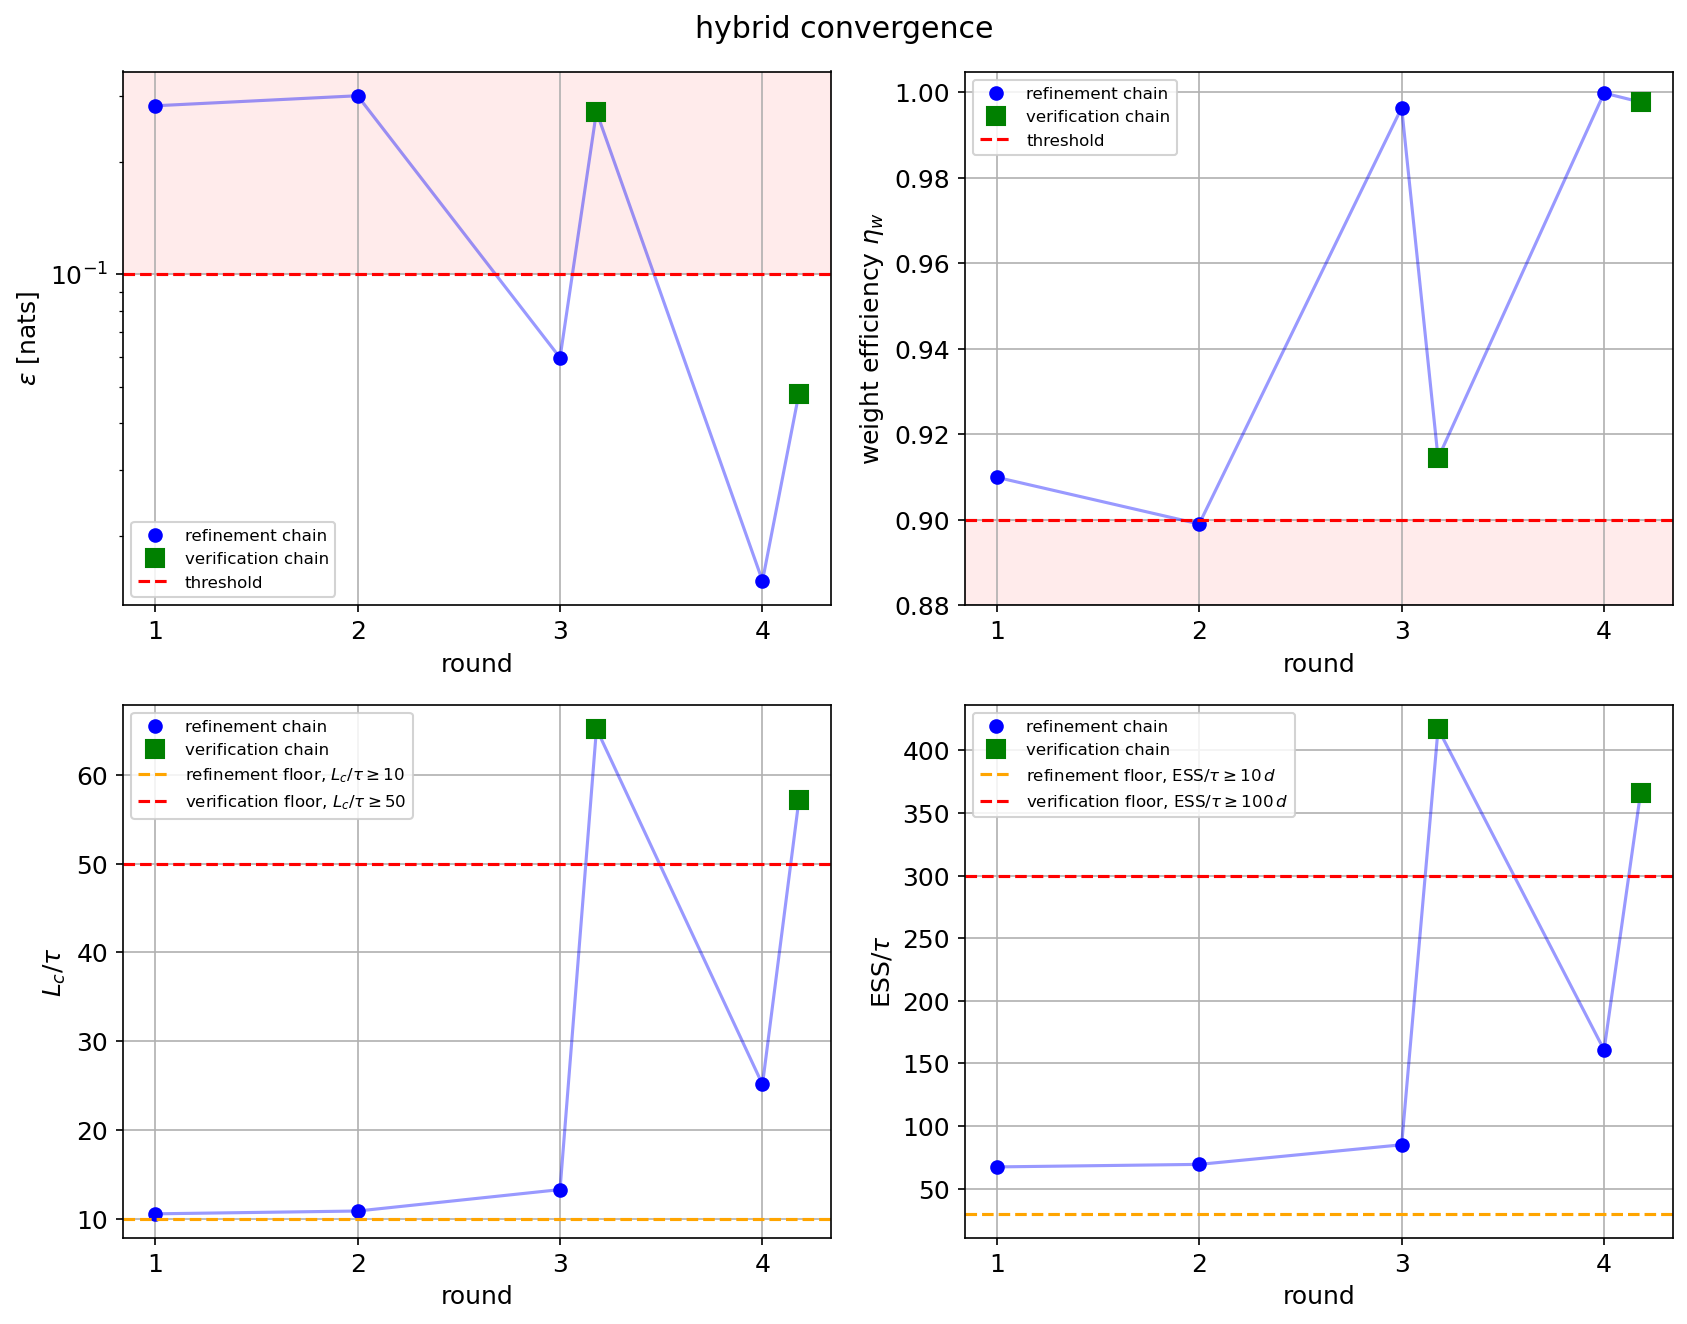
\includegraphics[width=0.8\linewidth]{example_mcmc_hybrid_convergence.png}
  \caption{Top: the criteria, surrogate accuracy $\varepsilon$ and weight efficiency $\effw$, with
           the region a converged run must stay out of shaded. The posterior shift is not tested in
           this run, so it has no panel. Bottom: how deeply the surrogate chain was sampled,
           $\Lc/\tau$ and ESS against their floors. Green squares are verification chains, blue
           circles refinement chains.}
  \label{fig:hybrid-convergence}
\end{figure}

\begin{center}
\small
\begin{tabular}{@{}lrrrrrrrr@{}}
  \toprule
  \textbf{round} & $n_{\mathrm{exp}}$ & $n_{\mathrm{train}}$ & $\varepsilon$ [nats] & $\effw$ & $\delta$ [sd] & $\Lc$ & $\Lc/\tau$ & ESS \\
  \midrule
  1  & 380    & 123 & 0.2824 & 0.910 & ---   & 360     & 10.5 & 67 \\
  2  & 580    & 323 & 0.3004 & 0.899 & 0.651 & 410     & 10.9 & 69 \\
  3  & 780    & 523 & 0.0599 & 0.996 & 0.277 & 454     & 13.3 & 85 \\
  3v &        &     & 0.2725 & 0.914 & 0.279 & 30\,154 & 65.2 & 417 \\
  4  & 1\,180 & 923 & 0.0152 & 1.000 & 0.200 & 5\,552  & 25.1 & 161 \\
  4v &        &     & 0.0480 & 0.998 & 0.210 & 65\,670 & 57.2 & 366 \\
  \bottomrule
\end{tabular}
\end{center}

\subsection{The posterior, round by round}

\begin{figure}[H]
  \centering
  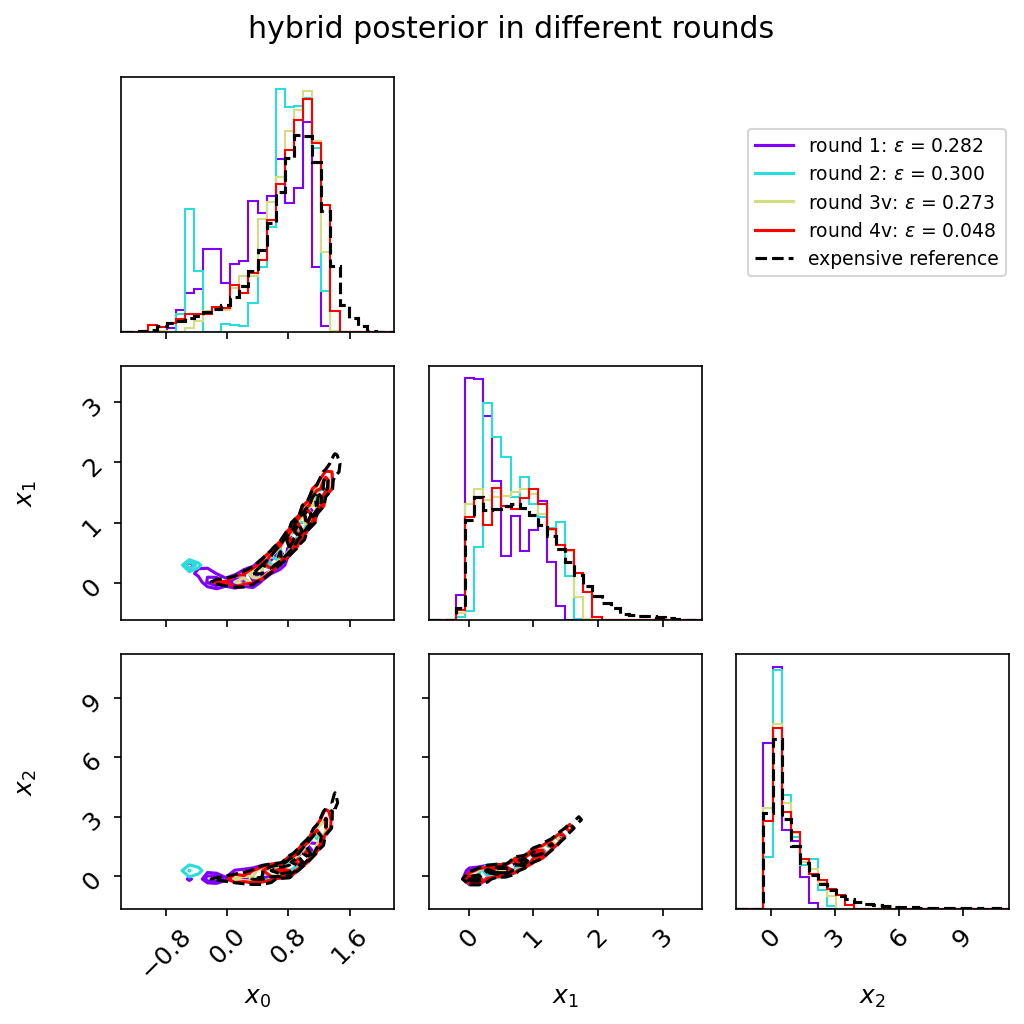
\includegraphics[width=0.82\linewidth]{example_mcmc_hybrid_hybrid_posterior_per_round.png}
  \caption{Each round's posterior as the pipeline left it --- for a verified round, the verification
           chain's --- one colour per round, with the expensive reference dashed in black.}
  \label{fig:hybrid-rounds}
\end{figure}

Round 1 ($\varepsilon = 0.28$) is visibly wrong: too low in all three parameters, with means
$(0.50, 0.47, 0.40)$ against the reference's $(0.80, 0.86, 1.12)$. From round 2 on the rounds follow
the reference's shape. The arm at negative $x_0$ comes and goes: the mass at $x_0 < -0.5$ is 2.2,
3.0, 0.1 and 2.5\% in rounds 1--4, against the reference's 2.1\%. What no round reaches is the other
end of the banana, the upper tails of $x_1$ and $x_2$ where the valley climbs steeply: the 99.5th
percentile of $x_1$ is at most 1.89, against the reference's 2.87. $\varepsilon$, being measured on
points drawn from the surrogate posterior, cannot see a region the chain never visits. The samples
behind the figure are kept in \code{work_dir/posteriors/posterior_round{k}.npy} when
\code{save_posterior_samples} is set; nothing else records them.

\subsection{Where the evaluations went}

\begin{figure}[H]
  \centering
  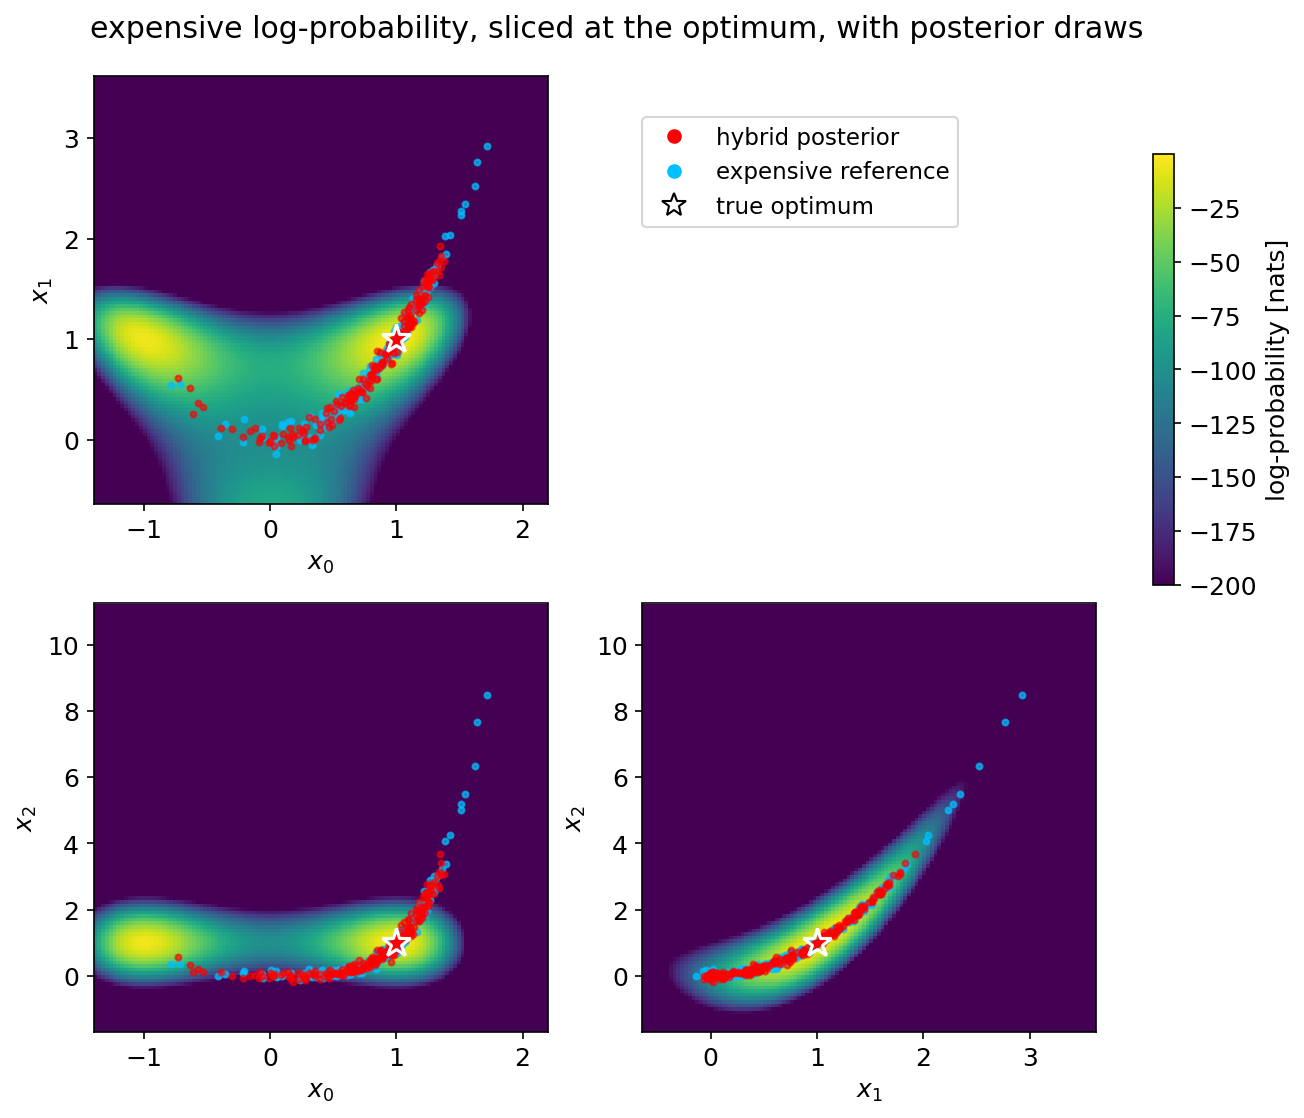
\includegraphics[width=0.96\linewidth]{example_mcmc_hybrid_log_prob_maps.png}
  \caption{The expensive log-probability in each parameter pair, with the remaining parameter held at
           the optimum, and 200 draws each from the hybrid posterior (red) and the reference (light
           blue). The colour scale is in nats, clipped 200 below the peak.}
\end{figure}

The two layers live in different spaces: the background is a \emph{slice} with the remaining
parameter pinned at the optimum, while the dots are a \emph{projection} of the full 3D posterior. A
bright patch with no dots on it, such as the lobe near $x_0 = -1$, is therefore not by itself evidence
of a missed mode. What does matter is visible in the top-left panel: the red draws follow the valley
along the arm at negative $x_0$ down to about $-0.9$, so this run did find it, but at the other end
they stop near $x_1 \approx 1.9$, where the reference continues to about 2.9.

\subsection{The posterior against the reference}

\begin{figure}[H]
  \centering
  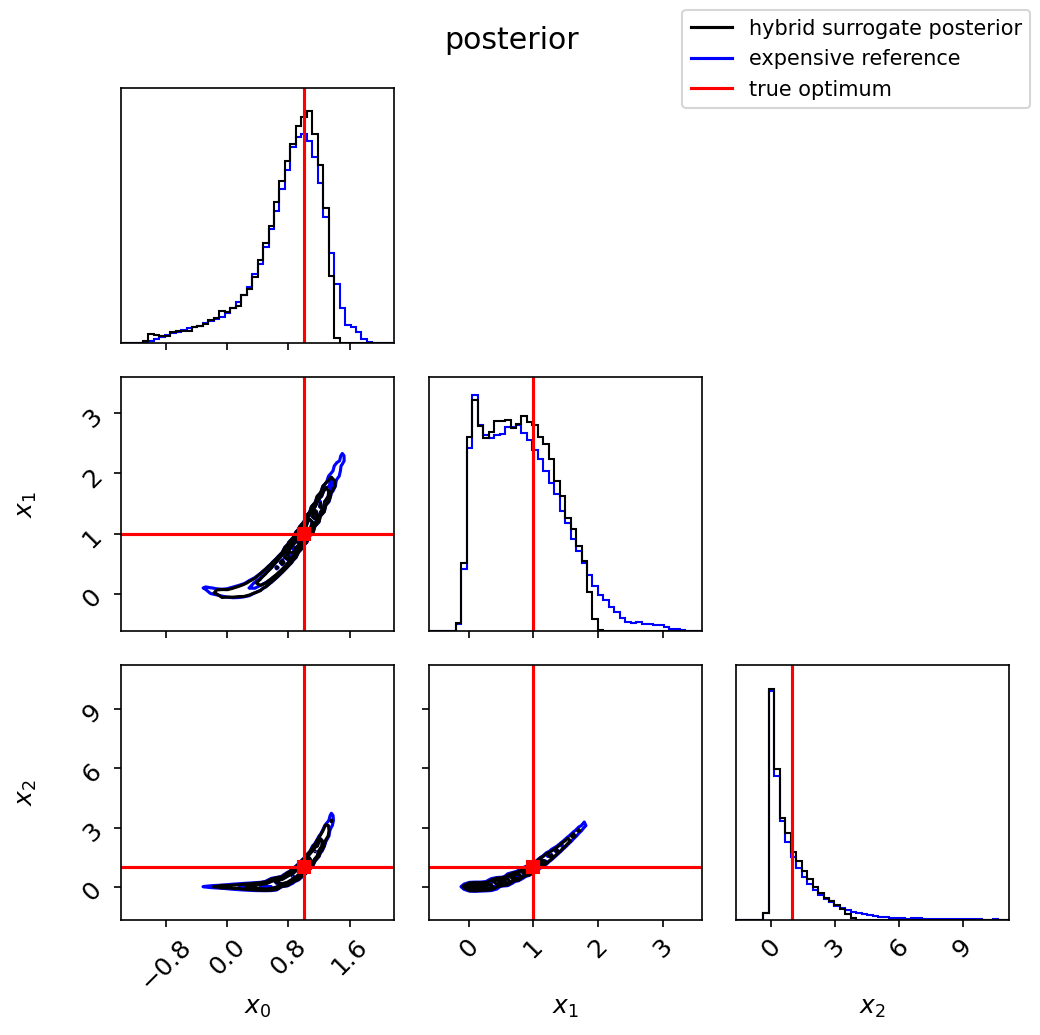
\includegraphics[width=0.82\linewidth]{example_mcmc_hybrid_posterior.png}
  \caption{The hybrid posterior (black) against the expensive reference (blue).}
\end{figure}

The centres agree to within 0.17 posterior widths, and the width in $x_0$ agrees too, 3\% narrower
than the reference's. The widths in $x_1$ and $x_2$ do not: the hybrid is 17\% and 37\% too narrow
there, far outside the reference's own uncertainty ($\pm 2.4\%$ and $\pm 5.8\%$, batch means over ten
blocks). The upper tails say why: $x_1 > 2$ and $x_2 > 4$ each hold $4.6\% \pm 0.6\%$ of the
reference's mass and none of the hybrid's. The run never sampled that end of the banana, so it never
scored it, and every criterion passed regardless.

\begin{cautionbox}[Reading hybrid widths]
Treat widths and tail quantities from a hybrid run as unconfirmed unless an independent expensive
chain checks them. Means are far more robust than tails.
\end{cautionbox}

\subsection{What the run writes}
\label{sec:hybrid-diagnostics}

For convenience, the run writes \code{work_dir/hybrid_diagnostics.txt} automatically. It is
rewritten in full every round, so a killed run still leaves its complete history and a resumed run
continues the same table. It is also written when a verification starts, with the refinement row and
a placeholder \code{<k>v verifying} row that the end of the round replaces, so a long verification
shows as such. It opens with the run's parameters, each \code{'auto'} with the value it resolved to,
and its expensive budget --- round 0, the regularization points, and what each round adds; here
$330 + 50 = 380$ points before the first fit, then 200 per round and 200 more per verification,
$380 + 4\times 200 + 2\times 200 = 1\,580$ in all. A legend describing every column follows, and
then the per-round table, shown here with four columns dropped to fit the page: \code{surrogate},
which names the class fitted that round and reads \code{DistributedGP} throughout here, and the
timings \code{t_valid_s}, \code{t_refresh_s} and \code{t_round_s} --- the validation batch, the
expensive refresh, and the round total.

\begin{lstlisting}[style=plain, basicstyle={\ttfamily\fontsize{7.6}{9.2}\selectfont}]
round n_expensive n_train w_log_err  w_eff post_shift shift_tol surr_iters  Lc/tau  ess/tau  t_fit_s t_mcmc_s
-------------------------------------------------------------------------------------------------------------
    1         380     123    0.2824  0.910        inf       off        360    10.5       67      2.3      2.4
    2         580     323    0.3004  0.899      0.651       off        410    10.9       69      3.3      3.3
    3         780     523    0.0599  0.996      0.277       off        454    13.3       85      7.6      4.3
   3v                        0.2725  0.914      0.279       off      30154    65.2      417             236.2
    4        1180     923    0.0152  1.000      0.200       off       5552    25.1      161     11.8     50.6
   4v                        0.0480  0.998      0.210       off      65670    57.2      366             588.3
\end{lstlisting}

Reading across a row:

\begin{itemize}
  \item \code{n_expensive} and \code{n_train} are the trim: what has been evaluated, and what
        entered the fit.
  \item \code{w_log_err}, \code{w_eff} and \code{post_shift} are the three criteria:
        $\varepsilon$ in nats, the weight efficiency $\effw$, and $\delta$ in posterior standard
        deviations. \code{post_shift} is computed and printed even when
        \code{posterior_shift_tolerance} is \code{None}, so it can be read after the fact.
        The \code{inf} of round 1 marks that there is no previous posterior to compare against yet.
        \code{shift_tol} is the tolerance applied to \code{post_shift}, the requested one raised to
        the noise floor; it reads \code{off} here, since the test is off.
  \item \code{surr_iters}, \code{Lc/tau} and \code{ess/tau} are how deeply the cheap chain was
        sampled: the length actually run, and what it bought in autocorrelation times and effective
        samples. A chain that keeps growing without clearing its floors shows it here.
  \item \code{t_fit_s} against \code{t_mcmc_s} is the pair worth watching. With experts of at
        most 500 points the fit stays cheap, 2.3\,s on 123 points to 11.8\,s on 923; here it is the
        sampling that dominates, 588.3\,s for the 65\,670 iterations of 4v. With a dense GP the
        balance tips the other way as the training set grows.
  \item A verified round prints two rows, $n$ and $n$v, and the columns they share ---
        \code{n_expensive}, \code{n_train}, \code{surrogate} and \code{t_fit_s} --- are left empty
        on the second: one fit, one training set, scored twice.
\end{itemize}

\section{Restarting, extending, and changing surrogate}

With \code{save_restart=True}, the restart file is written atomically after round 0 and after every
round, so a crash costs at most the round in progress. It is also written when a verification starts,
since that is usually the longest stretch of a round: a run stopped inside one keeps the refinement
batch it has already evaluated, and on resume redoes the round on the larger training set. It carries the whole training set, which also
makes it the cleanest way to \emph{extend} a finished run: raise \code{num_rounds_max} and resume
with \code{load_restart=True}.

The restart file stores only surrogate-agnostic state --- the training points and their values, the
evaluation count, the per-round diagnostics and the walker positions --- so the surrogate is rebuilt
from whatever is passed on resuming. A run whose fits have become too slow can be stopped and resumed
as an ensemble on the same training data:
\begin{lstlisting}
# start with the dense Gaussian process, for its accuracy
slurm_mcmc_hybrid(..., surrogate='gp', save_restart=True, work_dir='run17')

# fits too slow? stop it, and resume as an ensemble on the same data
from slurmcmc.hybrid import DistributedGPSurrogate
slurm_mcmc_hybrid(..., load_restart=True, save_restart=True, work_dir='run17',
                  num_rounds_max=40,
                  surrogate=DistributedGPSurrogate(max_points_per_expert=500,
                                                   parallel='joblib'))
\end{lstlisting}
Every combination works, in either direction, and the switch is recorded per round. With
\code{save_surrogate}, fitted surrogates are written to \code{work_dir/surrogates/surrogate_round{k}.pkl}:
\code{'latest'} keeps only the most recent, enough for a resumed round to skip its refit;
\code{'all'} keeps every round, at roughly $8n^2$ bytes each. A saved fit is reused only when the
round, the training-set size and the surrogate class all match.

Either mode also appends one line per fit to \code{work_dir/surrogates/surrogate_log.txt}: the
round, the surrogate class, how many points were accumulated, trimmed, subsampled and fitted, how
long the fit took, and the settings it was built with together with its fitted kernel. Being
appended rather than rewritten, it outlives \code{'latest'} pruning the pickles and continues
across a restart, so it is where a switch of surrogate --- or a fit that is becoming the bottleneck
--- shows up as a sequence.

\section{Results and warnings}

The returned dictionary contains the final posterior \code{samples}; \code{converged},
\code{num_rounds} and \code{num_expensive_evals}; per-round lists of every quantity that decided the
run, including \code{weighted_log_error_per_round}, \code{weight_efficiency_per_round},
\code{posterior_displacement_per_round},
\code{surrogate_iters_per_round}, \code{surrogate_tau_per_round}, \code{surrogate_ess_per_round},
\code{verified_per_round} and \code{blocking_criteria_per_round}, which names the criterion that held
each round back; \code{round_records}, one record per measurement including both rows of a verified
round; the fitted \code{surrogate}; the \code{validation_points} and \code{log_importance_weights}
of the final validation; and timings. The emulator's own uncertainty on the validation points,
\code{surrogate_std_per_round}, lets the common assumption that it is negligible be checked rather
than assumed.

Warnings are logged when posterior mass piles up against \code{param_bounds} or the confinement envelope, which can signal a
model error, an unidentifiable parameter or bounds set too tightly; and when a surrogate chain hits its
iteration cap short of its criteria.

\section{Argument reference}
\label{sec:hybrid-args}

Arguments shared with the other functions are in \cref{app:common}. The \emph{default} column is
what an omitted argument gets. Where that is \code{'auto'}, the setting is resolved for each run by a
rule in the number of parameters $d$, given in the description, and the diagnostics file prints
the value it resolved to (\cref{sec:hybrid-diagnostics}). \code{None}, where accepted, switches a
criterion or cap off. A \emph{recommendation} is advice for choosing a value, not a default. Settings
marked \emph{heuristic} have no derivation behind their value: they are reasonable starting points
that seldom need changing.

\subsubsection{Starting the run and its expensive budget}
\begin{argtable}
  \code{log_prob_fun} & required & the expensive log-probability; a callable or a deferred-import dictionary \\
  \code{init_points} & \code{None} & starting walkers of the round-0 MCMC, shape $(\Nc, d)$; required unless \code{initial_train_points} is given, and whenever \code{num_expensive_iters_per_round} $> 0$ \\
  \code{param_bounds} & \code{None} & a hard box that constrains the posterior; \code{None} runs unbounded (\cref{sec:unbounded}) \\
  \code{constraint_fun} & \code{None} & feasible when $\le 0$ \\
  \code{num_expensive_iters} & required & length of the round-0 MCMC, costing $(\text{iters}+1)\times\Nc$ evaluations, which become the initial training set. This is the user's budget, so it has no default: an error is raised if it is missing, unless \code{initial_train_points} is given, in which case it is unused. \code{0} is valid and evaluates only the starting walkers \\
  \code{initial_train_points}, \code{initial_train_values} & \code{None} & existing evaluations, shapes $(n, d)$ and $(n)$; round 0 is skipped \\
  \code{num_regularization_points} & \code{0} & points placed without reference to a posterior: uniform in the box, or around the training data when unbounded. Off by default because every one is an expensive evaluation. Recommendation: about $10\,d$ when the target may be multimodal or have mass far from \code{init_points}, since these are the only evaluations that can find it \\
  \code{num_validation_points} & \code{'auto'} & expensive evaluations per round, and the main per-round cost; they also join the training set. \code{'auto'} is $\max(200, 10\,d)$: 200 resolves $\varepsilon$ to about 5\% (its relative scatter is $\approx 1/\sqrt{2N}$) and $\effw$ to about $0.02$, and $10\,d$ is roughly the number of points a Gaussian process needs to resolve a $d$-dimensional region \\
  \code{num_rounds_max} & \code{100} & safety cap on the number of refinement rounds, meant to be large enough that convergence always ends the run first. It also bounds the worst-case budget, round 0 plus \code{num_rounds_max} validation batches, and one more batch per verification, so lower it if that is more than can be afforded \\
  \code{num_expensive_iters_per_round} & \code{0} & optional expensive MCMC each round, started from the surrogate posterior, costing $(\text{iters}+1)\times\Nc$ evaluations \\
\end{argtable}

\subsubsection{Surrogate and its sampling}
\begin{argtable}
  \code{surrogate} & \code{'gp'} & \code{'gp'}, \code{'polynomial'}, \code{DistributedGPSurrogate(...)}, or any object with \code{fit} and \code{predict} \\
  \code{polynomial_degree} & \code{2} & for \code{surrogate='polynomial'}; a quadratic is exact for a Gaussian posterior, and higher degrees extrapolate worse \\
  \code{surrogate_uncertainty_penalty} & \code{1.0} & $\kappa$ in $\mu - \kappa\sigma$, a one-standard-deviation lower bound (heuristic); \code{0} disables \\
  \code{num_surrogate_iters} & \code{'auto'} & length of the surrogate chain; \code{'auto'} sizes each chain from the $\tau$ of the one before (\cref{sec:two-depths}), the first from $\tau = 10\,d$, and extends it until the floors of its depth hold. An integer fixes only the starting length \\
  \code{max_surrogate_iters} & $10^6$ & absolute ceiling on a chain's length, a safety net only: a chain normally stops when its floors hold, or after two extensions in a row without progress in $\Lc/\tau$. \code{None} sets no ceiling \\
  \code{num_surrogate_walkers} & \code{'auto'} & walkers of the surrogate chain; \code{'auto'} is \texttt{emcee}'s minimum, $2d+2$, because at fixed work the ESS does not depend on the walker count while $\Lc/\tau$ falls with it \\
  \code{surrogate_burnin_fraction} & \code{0.2} & fraction of each chain discarded (a common convention) \\
  \code{refine_surrogate_ess}, \code{verify_surrogate_ess} & \code{'auto'}, \code{'auto'} & ESS floors of the two depths (\cref{sec:two-depths}); \code{'auto'} is $10\,d$ and $100\,d$, the two ends of the advised band. \code{None} demands no floor \\
  \code{refine_iters_per_tau}, \code{verify_iters_per_tau} & \code{'auto'}, \code{'auto'} & $\Lc/\tau$ floors of the two depths; \code{'auto'} is 10, the shortest chain whose own $\tau$ can be estimated, and 50, \texttt{emcee}'s rule for a reliable $\tau$. \code{None} demands no floor \\
  \code{max_verification_attempts} & \code{None} & rejections allowed before the run gives up; \code{None} is unlimited, since \code{num_rounds_max} bounds them anyway \\
\end{argtable}

\subsubsection{Convergence and training data}
\begin{argtable}
  \code{log_error_threshold} & \code{0.1} & $\varepsilon^\ast$ in nats, probability ratios accurate to about 10\%; tighten to 0.01--0.02 for tail quantities \\
  \code{min_weight_efficiency} & \code{0.9} & floor on $\effw$ of \cref{eq:weight-efficiency}, a fraction in $[0, 1]$: at most about 10\% of the surrogate posterior may lie where the target is negligible. A converged surrogate gives $\effw \approx e^{-\varepsilon^2} \approx 0.99$ at $\varepsilon = 0.1$ \\
  \code{posterior_shift_tolerance} & \code{None} & $\delta^\ast$ in posterior standard deviations, raised to the chains' noise floor where that is higher (\cref{eq:stability}); \code{None} does not test stability. Recommendation: 0.1, when the surrogate may still be improving between rounds \\
  \code{train_log_prob_trim_range} & \code{100.0} & trim points this many nats below the best; \code{None} disables. Safe up to $d \approx 50$: the posterior mass lies about $d/2 \pm \sqrt{d/2}$ nats below the peak, so raise it to about $2d$ beyond that \\
  \code{min_train_points_after_trim} & \code{'auto'} & the trim is skipped in a round where it would leave fewer points than this; \code{'auto'} is $10\,d$, what a Gaussian process needs, and at least the polynomial's $\binom{d+p}{p}$ coefficients for \code{surrogate='polynomial'}. \code{None} always trims, which can leave the fit with a handful of points if one evaluation lies far above the rest \\
  \code{max_train_points} & \code{None} & cap on the fit, by uniform random subsample \\
  \code{train_log_prob_floor} & \code{None} & absolute floor on training values \\
\end{argtable}

\needspace{8\baselineskip}  % keep the title with its table
\subsubsection{Saving}
\begin{argtable}
  \code{save_posterior_samples} & \code{None} & draws of each round's posterior kept as \code{work_dir/posteriors/posterior_round{k}.npy} \\
  \code{save_surrogate} & \code{None} & \code{'latest'} or \code{'all'} fitted surrogates, as \code{work_dir/surrogates/surrogate_round{k}.pkl} \\
  \code{restart_file} & \code{'hybrid_restart.pkl'} & name of the restart file in \code{work_dir} \\
  \code{expensive_mcmc_kwargs} & \code{None} & forwarded to the expensive \code{slurm_mcmc} runs \\
\end{argtable}
